%%%%%%%%%%%%%%%%%%%%%%%%%%%%%%%%%%%%%%%%%%%%%%%%%%%%%%%%%%%%%%%%%%%%%%
% Overleaf (WriteLaTeX) Example: Molecular Chemistry Presentation
%
% Source: http://www.overleaf.com
%
% In these slides we show how Overleaf can be used with standard 
% chemistry packages to easily create professional presentations.
% 
% Feel free to distribute this example, but please keep the referral
% to overleaf.com
% 
%%%%%%%%%%%%%%%%%%%%%%%%%%%%%%%%%%%%%%%%%%%%%%%%%%%%%%%%%%%%%%%%%%%%%%

\documentclass{beamer}

\mode<presentation>
{
  \usetheme{Madrid}       % or try default, Darmstadt, Warsaw, ...
  \usecolortheme{default} % or try albatross, beaver, crane, ...
  \usefonttheme{default}    % or try default, structurebold, ...
  \setbeamertemplate{navigation symbols}{}
  \setbeamertemplate{caption}[numbered]
} 

\usepackage[english]{babel}
\usepackage[utf8x]{inputenc}
\usepackage{graphicx}
\usepackage{hyperref}
  \hypersetup{colorlinks=true}
  \hypersetup{urlcolor=blue}
  \hypersetup{linkcolor = .}
\usepackage{xcolor}
\usepackage{siunitx}
  \sisetup{separate-uncertainty = true}
\usepackage{physics}
\usepackage[font=small,labelfont=bf]{caption}
\usepackage{subcaption}
\usepackage[en-GB]{datetime2}
\usepackage{overpic}
\usepackage{feynmp}
\DeclareGraphicsRule{*}{mps}{*}{}
\usepackage{scalerel}
\newcommand{\mylbrace}[2]{\vspace{#2pt}\hspace{6pt}\scaleleftright[\dimexpr5pt+#1\dimexpr0.06pt]{\lbrace}{\rule[\dimexpr2pt-#1\dimexpr0.5pt]{-4pt}{#1pt}}{.}}
\newcommand{\myrbrace}[2]{\vspace{#2pt}\scaleleftright[\dimexpr5pt+#1\dimexpr0.06pt]{.}{\rule[\dimexpr2pt-#1\dimexpr0.5pt]{-4pt}{#1pt}}{\rbrace}\hspace{6pt}}

% Here's where the presentation starts, with the info for the title slide
\title[TORCH meeting]{PID studies with proto-TORCH testbeam update\\TORCH meeting}

\author{Martin Tat}
\institute{University of Oxford}
\date{18th July 2022}

\titlegraphic{
\includegraphics[height = 2cm]{lhcb.jpg}\hspace{2cm}~%
              
\includegraphics[height = 2cm]{OxfordLogo.pdf}}

\begin{document}

\begin{frame}
  \titlepage
\end{frame}

% These three lines create an automatically generated table of contents.
%\begin{frame}{Outline}
%  \tableofcontents
%\end{frame}

\section{Introduction}
\begin{frame}{Introduction}
  \begin{itemize}
    \setlength\itemsep{1.0em}
    \item{What I presented last time:}
    \begin{itemize}
      \setlength\itemsep{0.5em}
      \item{Study of likelihood calculation with particle gun simulations}
      \item{Initial studies of reconstruction and PID separation power in proto-TORCH testbeam data}
      \item{Need a better understanding of discrepancies between simulation and data}
    \end{itemize}
    \item{Today's presentation: Quick progress update}
    \item{Long term goal:}
    \begin{itemize}
      \setlength\itemsep{0.5em}
      \item{Prepare for PID study of next testbeam data}
    \end{itemize}
  \end{itemize}
\end{frame}

\section{Recap from previous presentation}
\begin{frame}{Beam position}
  \begin{figure}
    \centering
    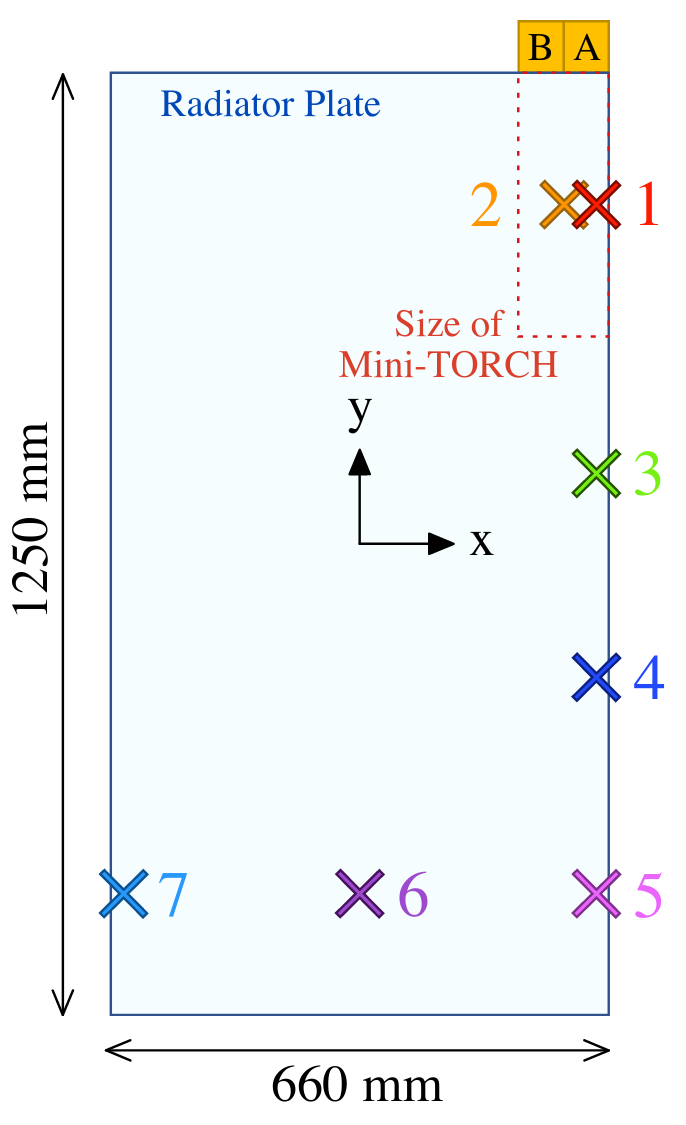
\includegraphics[width = 0.35\textwidth]{Plots/BeamPosition.png}
  \end{figure}
  \begin{center}
    \large Have only studied position 1 so far
  \end{center}
\end{frame}

\begin{frame}{Simulated hit maps}
  \begin{figure}
    \centering
    \vspace{-0.2cm}
    \begin{subfigure}{0.5\textwidth}
      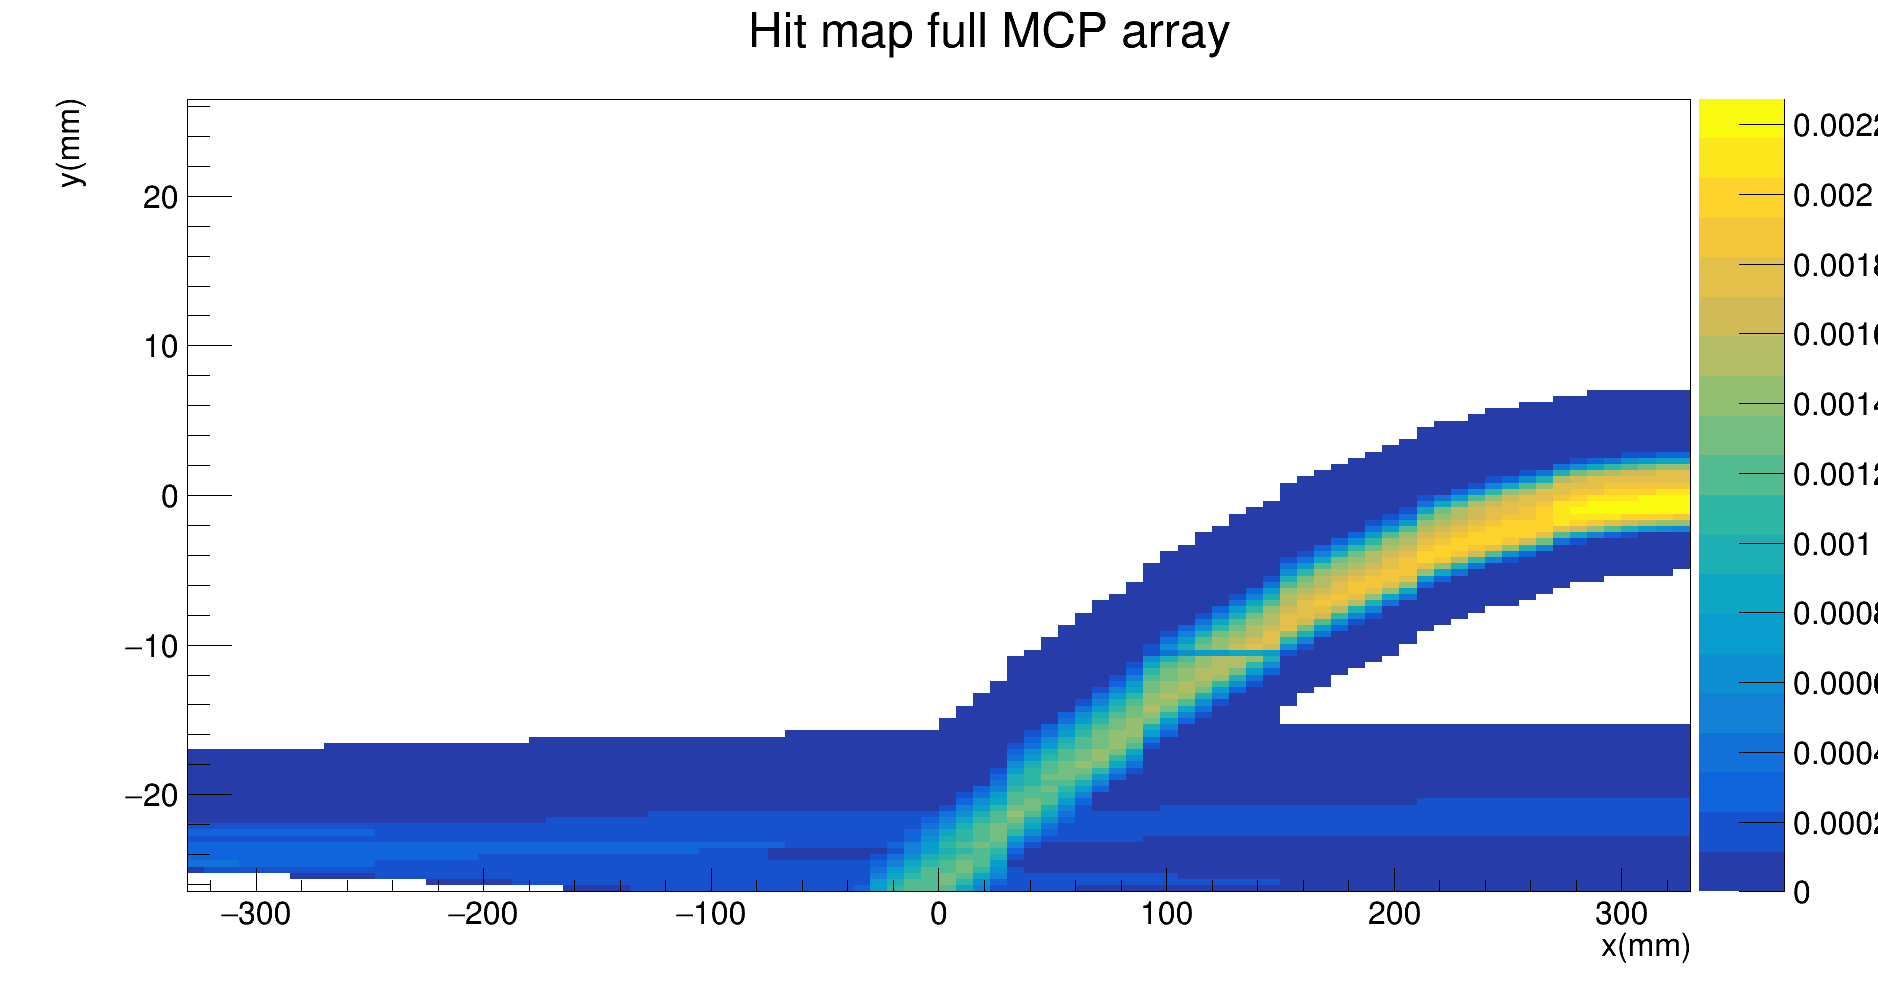
\includegraphics[width = 1.0\textwidth]{Plots/HitMapMCPFull.png}
      \caption{Full MCP array, nominal QE}
    \end{subfigure}%
    \begin{subfigure}{0.5\textwidth}
      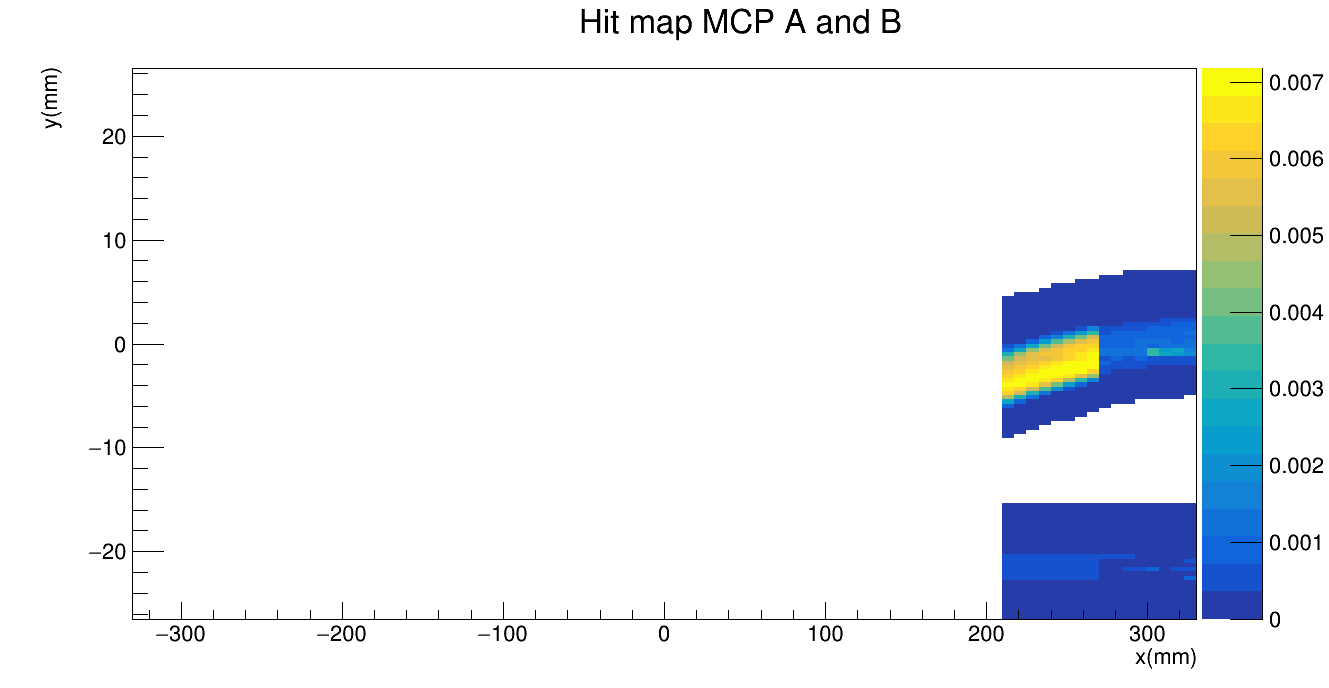
\includegraphics[width = 1.0\textwidth]{Plots/HitMapMCPAB_CorrectOrder.png}
      \caption{MCP (reduced QE) A and B}
    \end{subfigure}
    \caption{Track incident on top right corner (position 1)}
  \end{figure}
  \begin{center}
    \Large For now I will only study MCP-B
  \end{center}
\end{frame}

\begin{frame}{Likelihood calculation}
  \begin{itemize}
    \item{Probability of photon hit with energy $E_\gamma$, azimuthal angle $\phi_c$, time $t_0$:}
  \end{itemize}
  \begin{align*}
    P(E_\gamma, \phi_c, z, t_0) =& P(\phi_c)P(z)P(t_0)P(E_\gamma)\Theta(E_\gamma, \phi_c, z) \\
    =& \frac{1}{2\pi}\frac{1}{r_z}P(E_\gamma)P(t_0)\Theta(E_\gamma, \phi_c, z)
  \end{align*}
  \begin{itemize}
    \item{Transform to detector coordinates $(x_d, y_d)$:}
  \end{itemize}
  \begin{equation*}
    P(x_d, y_d, t_d) = P(E_\gamma, \phi_c, t_0)/\lvert J\rvert, \quad \lvert J\rvert = \Big\lvert\frac{\partial y_d}{\partial E_\gamma}\frac{\partial x_d}{\partial\phi_c} - \frac{\partial x_d}{\partial E_\gamma}\frac{\partial y_d}{\partial\phi_c}\Big\rvert
  \end{equation*}
  \begin{itemize}
    \item{$P(t_0)$: Gaussian PDF with $\sim\SI{70}{\pico\second}$ time resolution}
    \item{$P(E_\gamma)$: Frank-Tamm formula}
  \end{itemize}
  \begin{itemize}
    \item{PID algorithm described in \href{https://www.overleaf.com/project/5d0b9c5a5005405666aacd05}{LHCb-PUB-2022-007}}
  \end{itemize}
\end{frame}

\begin{frame}{PID efficiency simulation}
  \begin{figure}
    \centering
    \vspace{-0.2cm}
    \begin{subfigure}{0.5\textwidth}
      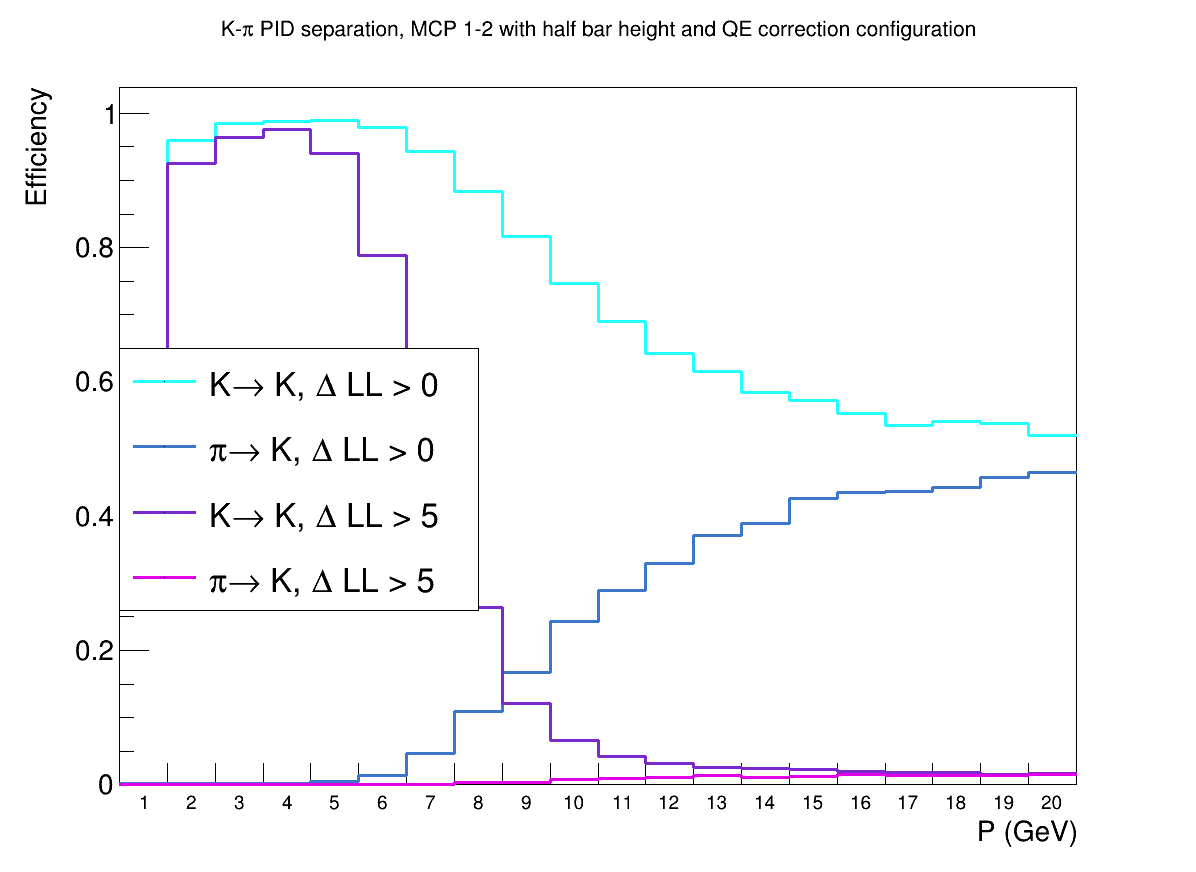
\includegraphics[width = 1.0\textwidth]{Plots/KaonPionPIDEfficiencyStandardMCPAB.png}
      \caption{Kaon-pion}
    \end{subfigure}%
    \begin{subfigure}{0.5\textwidth}
      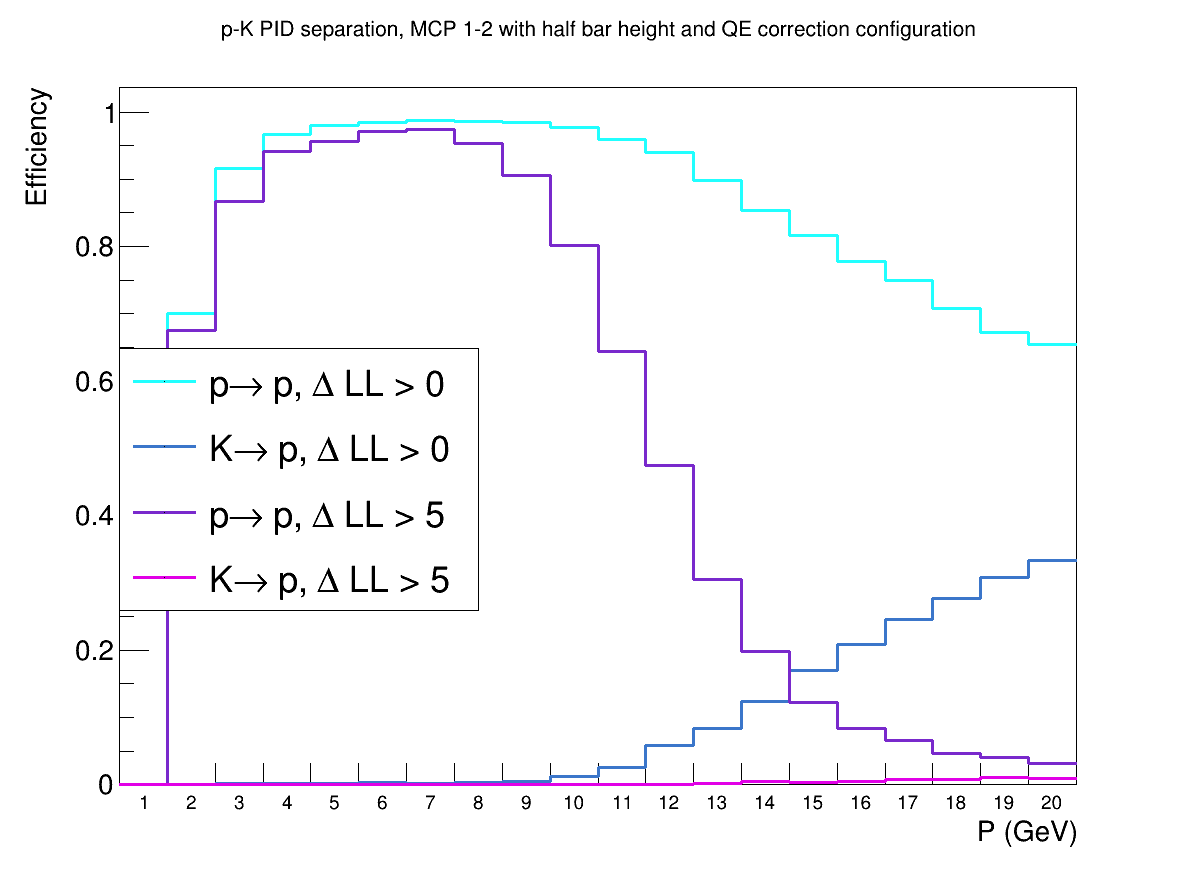
\includegraphics[width = 1.0\textwidth]{Plots/PionProtonPIDEfficiencyStandardMCPAB.png}
      \caption{Kaon-proton}
    \end{subfigure}
    \caption{PID efficiency}
  \end{figure}
\end{frame}

\begin{frame}{Likelihood in proto-TORCH testbeam data}
  \begin{figure}
    \centering
    \vspace{-0.2cm}
    \begin{subfigure}{0.5\textwidth}
      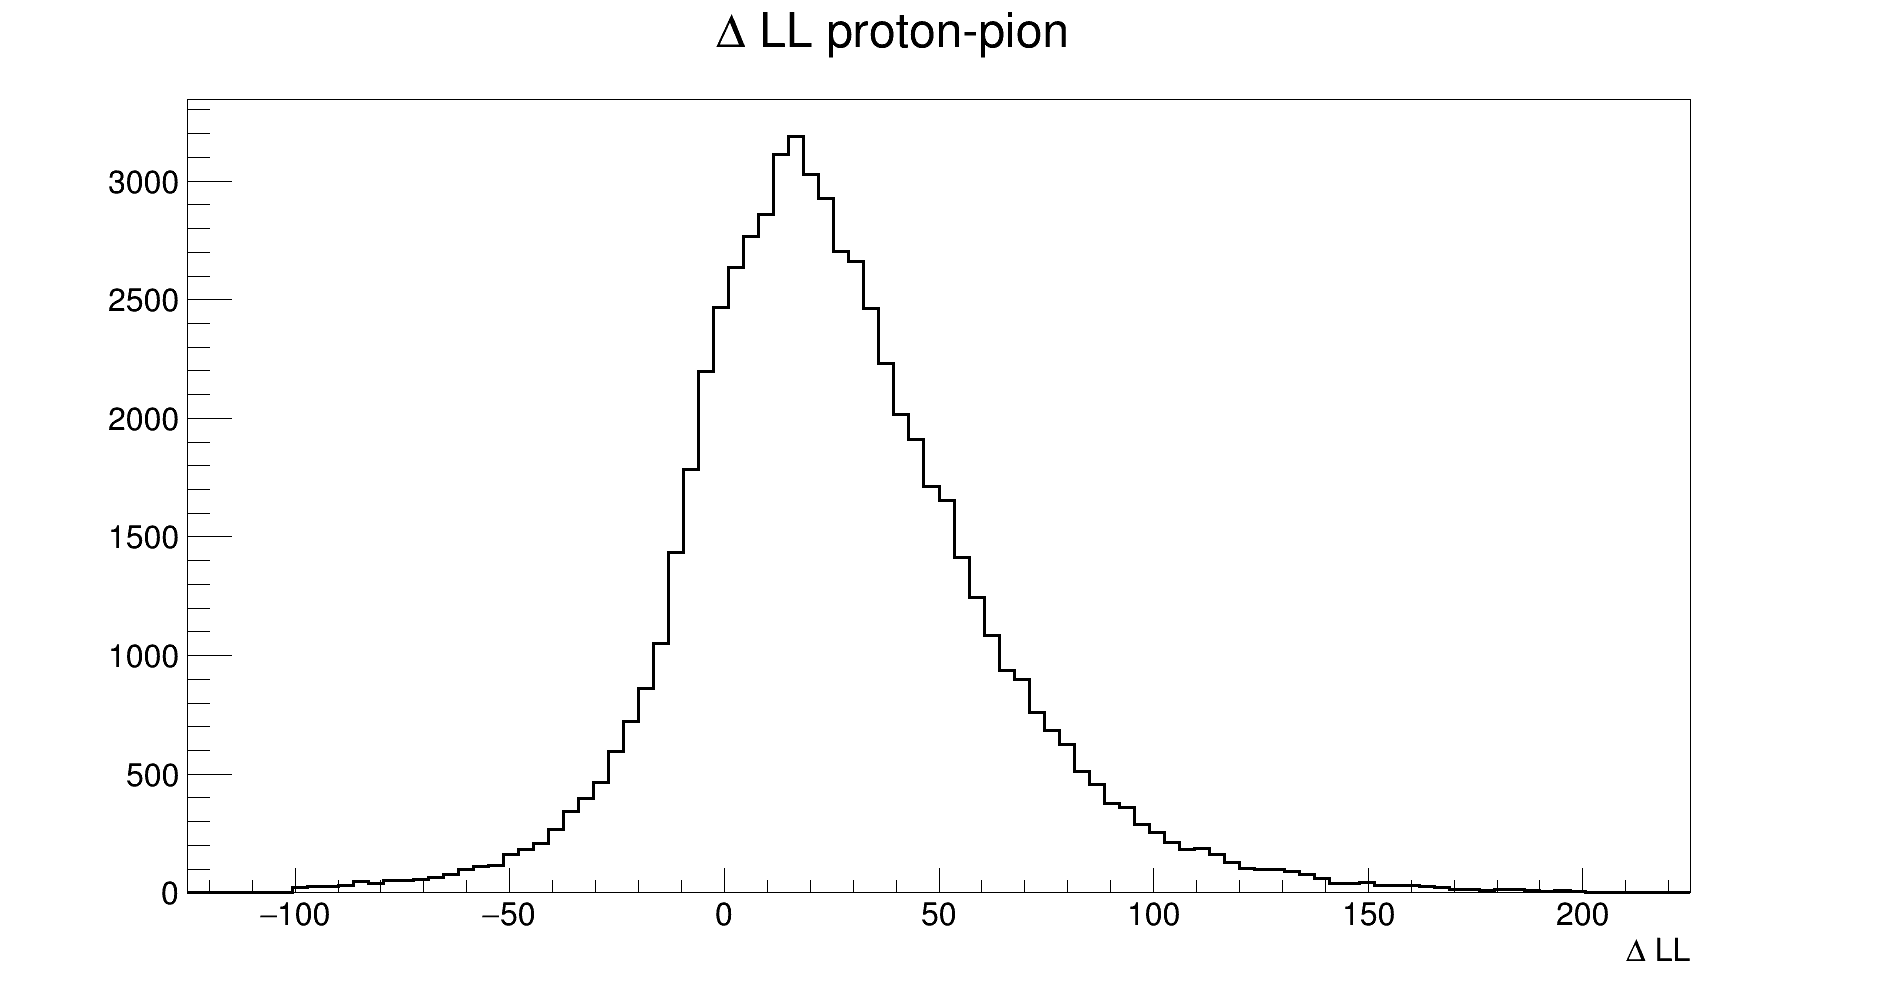
\includegraphics[width = 1.0\textwidth]{Plots/TestBeamDLLPion.png}
      \caption{Pion sample}
    \end{subfigure}%
    \begin{subfigure}{0.5\textwidth}
      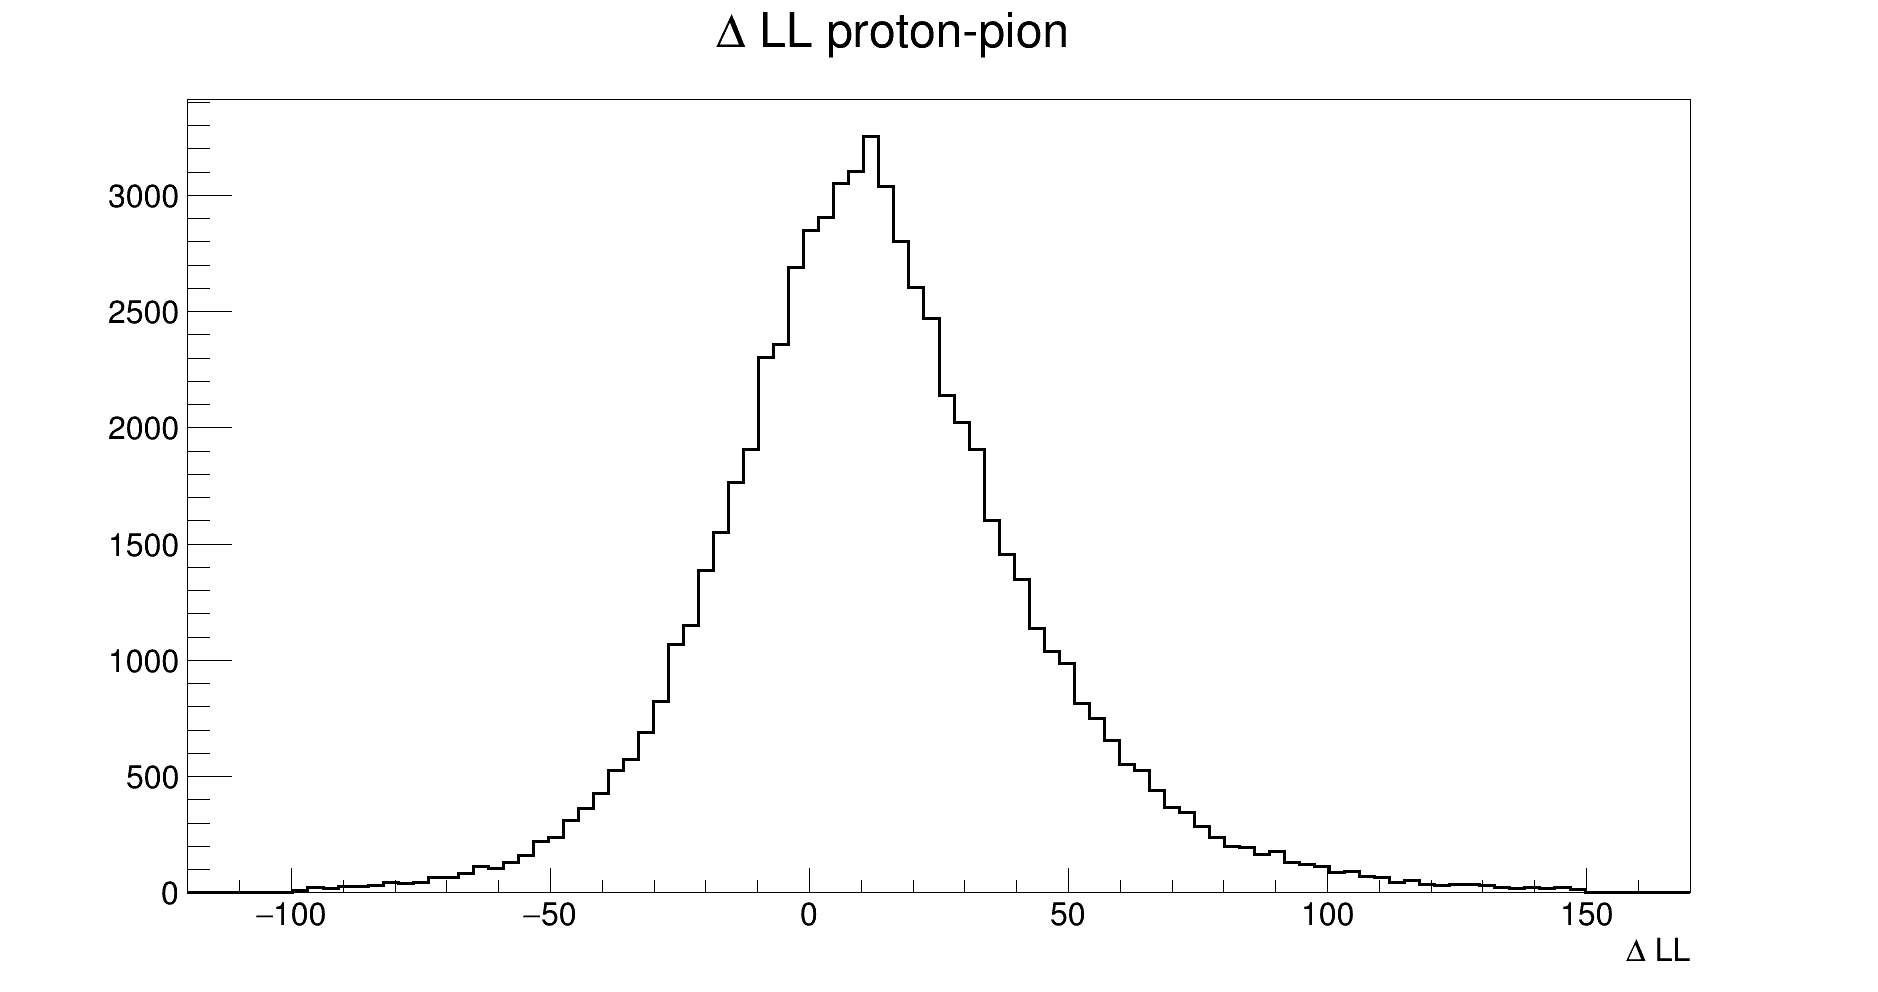
\includegraphics[width = 1.0\textwidth]{Plots/TestBeamDLLProton.png}
      \caption{Proton sample}
    \end{subfigure}
    \caption{$\Delta{\rm LL}$ of testbeam data}
  \end{figure}
  \begin{center}
    \large Results ``out of the box'' at $\SI{8}{\giga\eV}$: \\
    \large Pion efficiency: $78.6\%$ \\
    \large Proton efficiency: $66.9\%$
  \end{center}
\end{frame}

\section{Why was the proton PID performance much worse?}
\begin{frame}{Why was the proton PID performance much worse?}
  \begin{itemize}
    \setlength\itemsep{1.0em}
    \item{Main issue: Calibration between MCP columns}
    \begin{itemize}
      \item{Solution: Need to time align each MCP column in data with simulation}
    \end{itemize}
    \item{Additionally: Need to account for travel time difference from TORCH to T2}
    \item{After accounting for these effects, the proton PID efficiency improved:}
    \begin{itemize}
      \item{Pion efficiency: $82.7\%$}
      \item{Proton efficiency: $79.0\%$}
    \end{itemize}
  \end{itemize}
\end{frame}


\section{Why is the performance in simulation so good?}
\begin{frame}{Why is the performance in simulation so good?}
  \begin{itemize}
    \setlength\itemsep{1.0em}
    \item{A few small effects that should be accounted for:}
    \begin{itemize}
      \item{Time resolution is simulation is too good ($\SI{55}{\pico\second}$)}
      \item{Each MCP column can have a different time resolution}
      \item{Solution: Convolve time distribution from simulation with Gaussian and fit to testbeam data}
    \end{itemize}
    \item{A very large effect that must be accounted for:}
    \begin{itemize}
      \item{Backscattering results in a very large tail in the testbeam time distribution}
      \item{Strategy: Convolve time distribution with a Crystal Ball instead of Gaussian}
    \end{itemize}
  \end{itemize}
\end{frame}

\begin{frame}{Why is the performance in simulation so good?}
  \begin{itemize}
    \setlength\itemsep{0.0em}
    \item{In summary:}
    \begin{enumerate}
    \setlength\itemsep{0.0em}
      \item{Separate all MCP columns in data and simulation}
      \item{Convolve time distribution in simulation with Crystal Ball}
      \item{Fit each MCP column in data separately}
      \item{Use Crystal Ball position for time calibration, width for resolution effects and tails for backscattering effects}
    \end{enumerate}
  \end{itemize}
  \begin{figure}
    \centering
    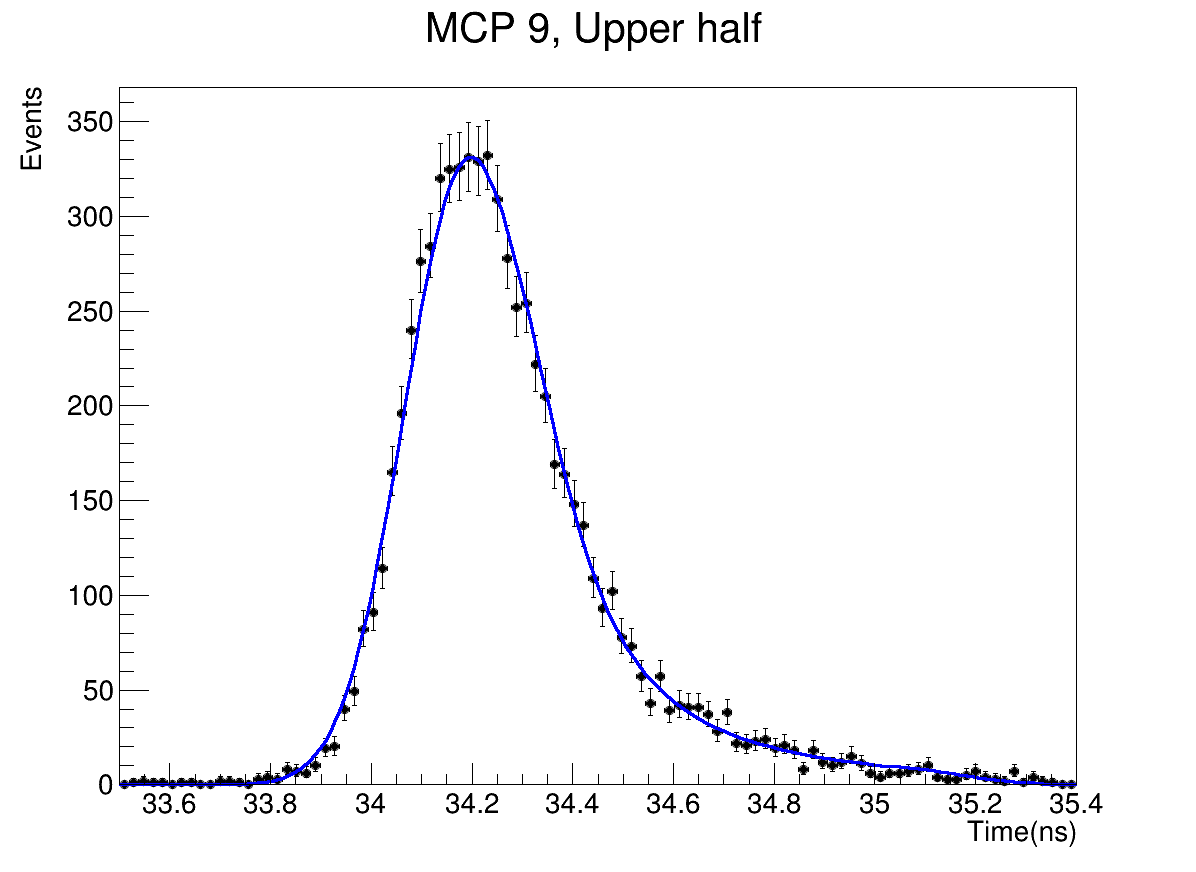
\includegraphics[width = 0.6\textwidth]{Plots/Example_Time_alignment.png}
  \end{figure}
\end{frame}

\section{Results after adding these effects}
\begin{frame}{PID efficiency simulation}
  \begin{figure}
    \centering
    \vspace{-0.2cm}
    \begin{subfigure}{0.5\textwidth}
      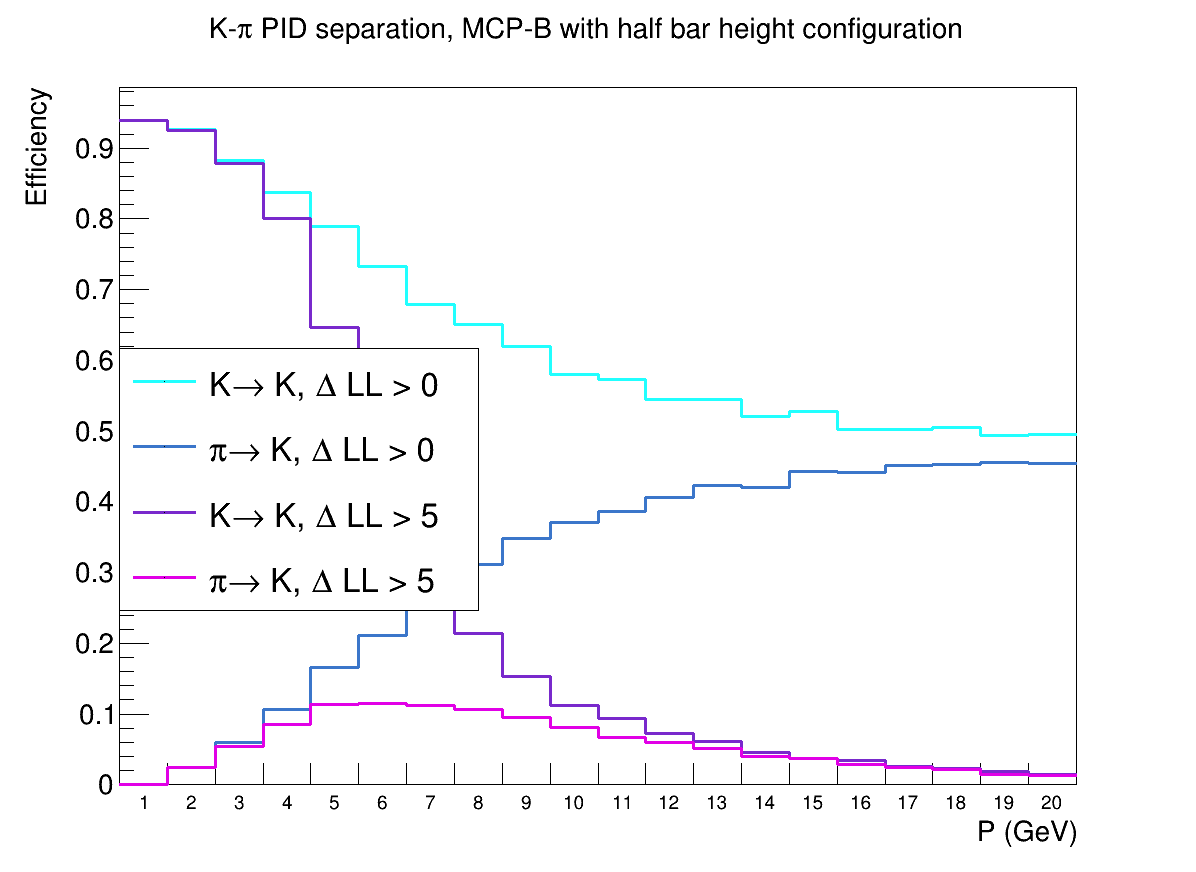
\includegraphics[width = 1.0\textwidth]{Plots/KaonPionPIDEfficiencyMCPB_Backscattering.png}
      \caption{Kaon-pion}
    \end{subfigure}%
    \begin{subfigure}{0.5\textwidth}
      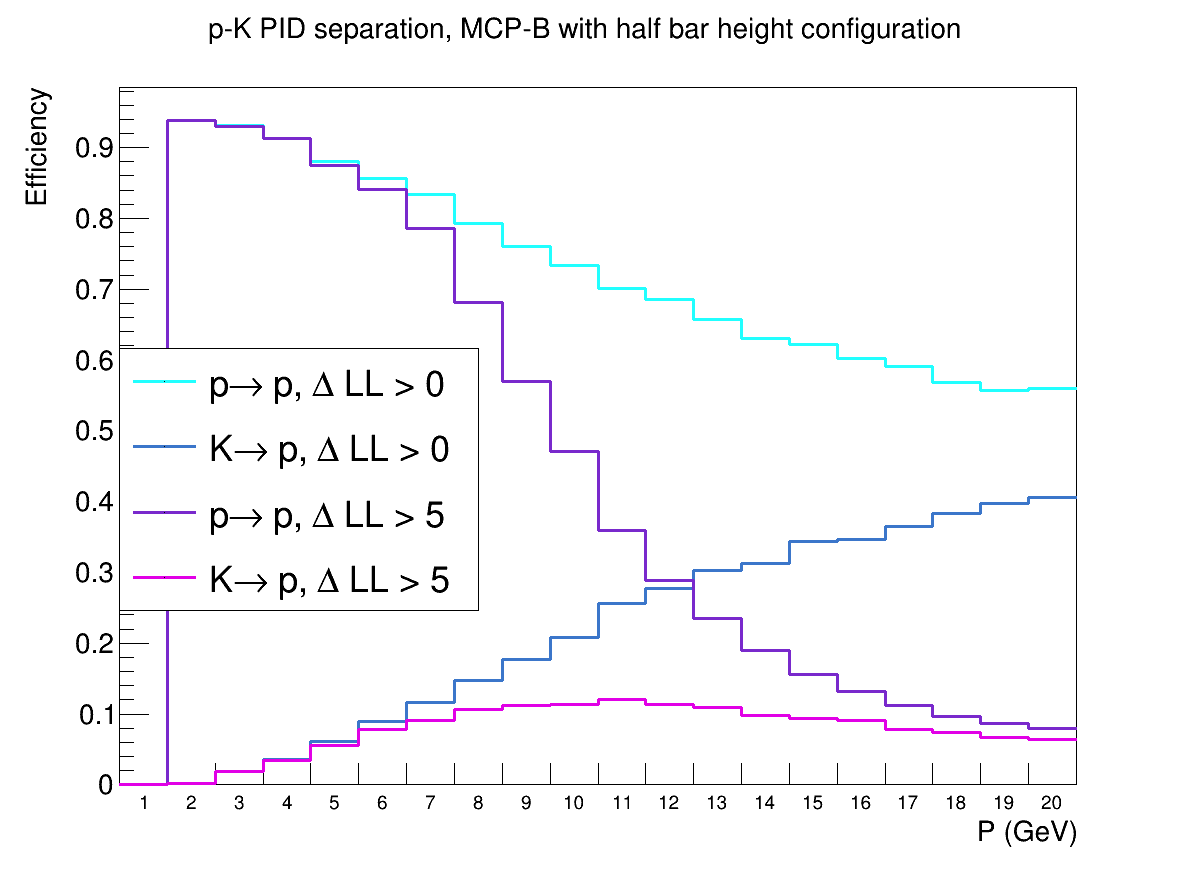
\includegraphics[width = 1.0\textwidth]{Plots/ProtonKaonPIDEfficiencyMCPB_Backscattering.png}
      \caption{Kaon-proton}
    \end{subfigure}
    \caption{PID efficiency}
  \end{figure}
\end{frame}

\begin{frame}{PID efficiency in testbeam}
  \begin{figure}
    \centering
    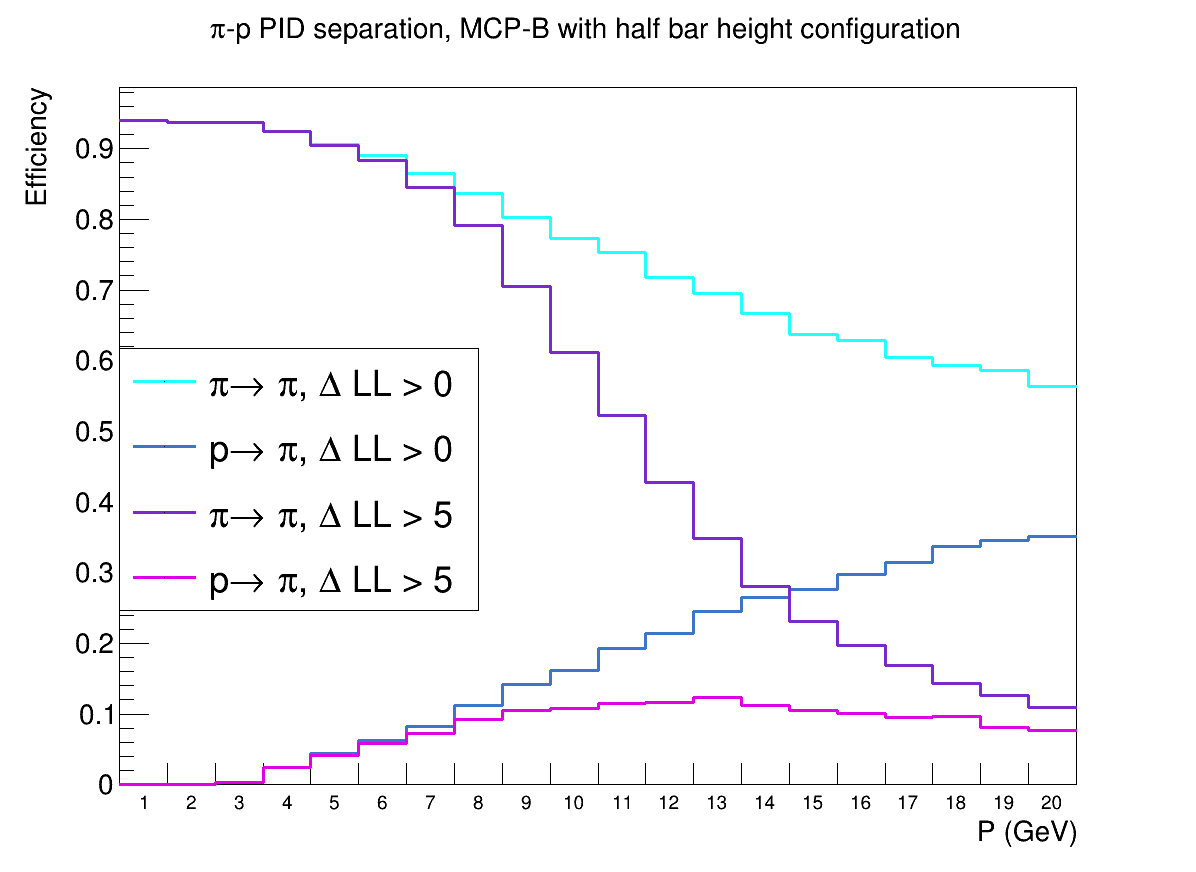
\includegraphics[width = 0.5\textwidth]{Plots/PionProtonPIDEfficiencyMCPB_Backscattering.png}
    \caption{Pion-proton PID efficiency}
  \end{figure}
  \begin{center}
    \begin{tabular}{lcccccc} 
      \hline
      Sample        & Testbeam data & Simulation & Without backscattering \\
      \hline
      Pion sample   & $82.7\%$      & $85.5\%$   & $99.0\%$ \\
      Proton sample & $79.0\%$      & $84.6\%$   & $98.7\%$ \\
      \hline
    \end{tabular}
  \end{center}
\end{frame}

\begin{frame}{Likelihod distributions in testbeam and simulation}
  \begin{figure}
    \centering
    \vspace{-0.2cm}
    \begin{subfigure}{0.5\textwidth}
      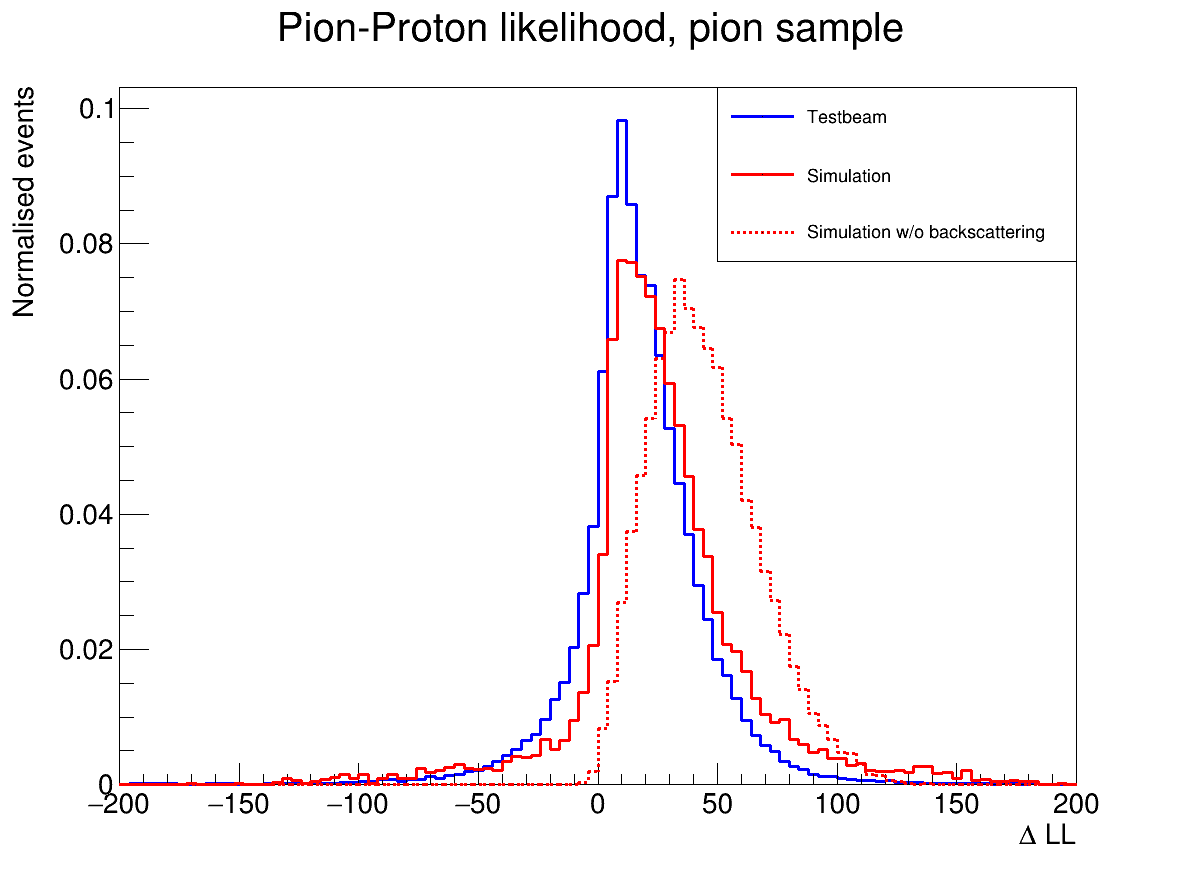
\includegraphics[width = 1.0\textwidth]{Plots/Pion_likelihood_comparison.png}
      \caption{Pion sample}
    \end{subfigure}%
    \begin{subfigure}{0.5\textwidth}
      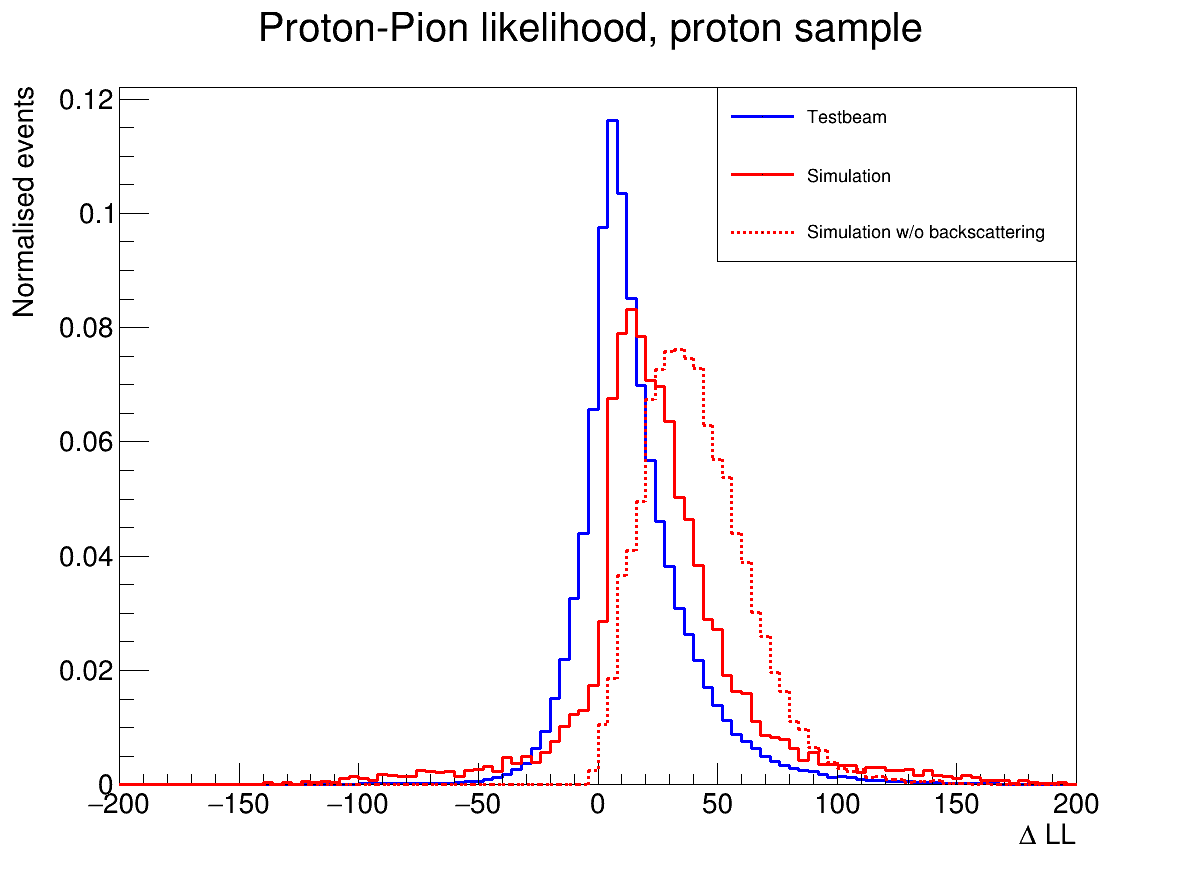
\includegraphics[width = 1.0\textwidth]{Plots/Proton_likelihood_comparison.png}
      \caption{Proton sample}
    \end{subfigure}
    \caption{Likelihood distributions}
  \end{figure}
  \begin{center}
    \large Not perfect agreement, but much better now
  \end{center}
\end{frame}

\section{Summary}
\begin{frame}{Summary}
  \begin{itemize}
  \setlength\itemsep{1.0em}
    \item{Discrepancies between PID efficiencies in data and simulation previously}
    \item{Two main effects:}
    \begin{enumerate}
      \item{Time calibration of individual MCP columns}
      \item{Backscattering results in large tail in time distribution}
    \end{enumerate}
    \item{Smear simulation with Crystal Ball shape}
    \item{Agreement much better now!}
  \end{itemize}
  \begin{center}
    \Huge Thank you for listening!
  \end{center}
\end{frame}

\end{document}